\label{sec:mcnp}
\section{MCNP}
\subsection{General information}
MCNP, or Monte-Carlo N-Particle Transport Code, is a software package that is used for nuclear simulations. It is based on Fortran, the most common version being Fortran-90. A typical MCNP program contains definitions for geometries in a 3D dimensional Cartesian coordinate system, which are composed of cells, surfaces and their material definitions. In figure \ref{fig:regions}, A and B are two surfaces defined in MCNP. Each surface has a negative and positive value, which is important for particle interaction. If a value is negative, then the surface is facing inwards relative to the origin. The mathematical depiction can be seen in figure \ref{fig:planes}, where the normal vector $n_2$ is expressed by a negative surface number, whilst the vector $n_1$ is a positive surface number.
\begin{figure}[!htbp]
\caption{Normal vectors to a plane.}
\label{fig:planes}
\centering
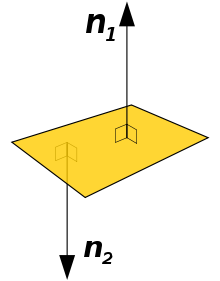
\includegraphics[width=0.25\textwidth]{normals.png}
\end{figure}
Surfaces can be combined together to create cells. Defined as either unions or intersections, the resulting cells from surfaces A and B are seen in figure \ref{fig:regions}. An important MCNP concept to remember is that when looking at a typical geometrical shape, for example a cube, one must double the number of faces. In a cube, the number of faces is 6, however, because of positive and negative surfaces, the shape should be looked at as having 12 faces. Understanding this was a key point in the project. Being able to identify which regions were required and which surfaces to ignore allowed us to carry out simulations more effectively and accurately.
\begin{figure}[!htbp]
\caption{Example MCNP regions.}
\label{fig:regions}
\centering
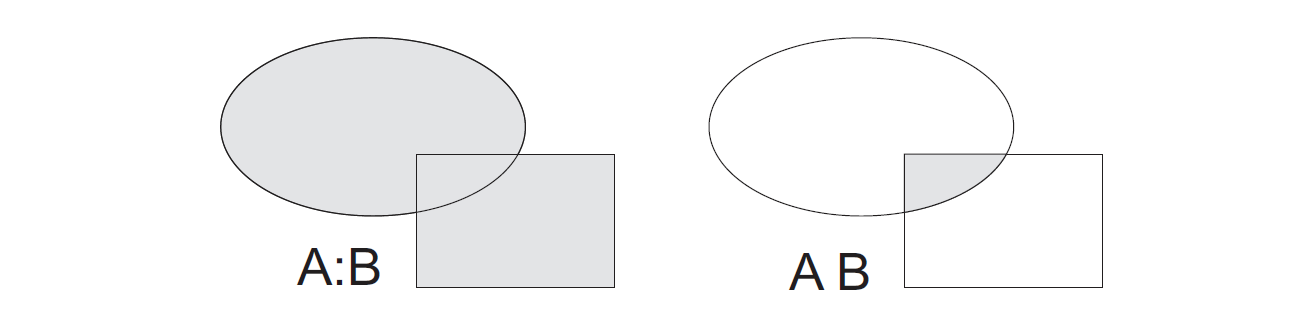
\includegraphics[width=0.75\textwidth]{regions.png}
\end{figure}
A sample MCNP input file consists of the following components. There are 3 blocks, each separated by a blank line: first come the cell definitions, followed by surface definitions and finally the data blocks (introduced in section \ref{sec:simulations}). There are also optional comments that can be added at different points. The blank lines, however, need to be kept, otherwise MCNP will not be able to distinguish the blocks. A full line comment starts with the letter "c", whilst an inline comment starts with a dollar sign (\$). It is important to note that all lines should not exceed 80 characters in length. A visual representation of an MCNP program can be see in figure \ref{fig:program}
\begin{figure}[!htbp]
\caption{MCNP program structure.}
\label{fig:program}
\centering
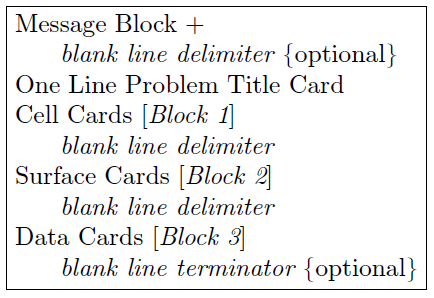
\includegraphics[width=0.75\textwidth]{prog.png}
\end{figure}
\subsection{Example geometry}
A good way to understand MCNP syntax and its complexity is a simple example. As a result, a graphite cube will be submerged into a spherical container and that container will be filled with water. Throughout the project, it was found that specifying surfaces first was an easier approach, followed up the cell definitions. As a result, the input file was structured out of order, however, this allowed for a more step-by-step approach to the simulation setup. In order to create a cube, the general procedure is the following:
\begin{enumerate}
	\item Specify 6 outward facing surfaces.
	\item Specify 6 inward facing surfaces.
	\item Combine all of the relevant surfaces into a cell. For example, the outside of the cube would be a union of the outward facing surfaces, and the inside will be a union of the inward facing ones.
\end{enumerate}
Although this is only 3 steps, the procedure is fairly complex. In order to specify a single surface of a cube, one must figure out the side length, center and boundaries of the square in question. Doing this 12 times in a 3D coordinate system becomes monotone and challenging, especially when dealing with complex, irregular geometries. MCNP does have a solution, however - macrobodies. With one command, MCNP will know that the shape specified is a cube, sphere or pyramid (to name a few). The command for a rectangular parallelepiped is \textbf{RPP}. In order to create a cube centered at the origin with a side length of $10$cm, the command is:
\begin{center}
\begin{tabular}{c}
\begin{lstlisting}
10 RPP -5 5 -5 5 -5 5
\end{lstlisting}
\end{tabular}
\end{center}
In the above example, 10 is the number of the macrobody, which will be important in the cell block. The first two numbers indicate a starting and ending x-coordinate\footnote{MCNP units are metric, with length defaulting to centimeters.}, followed by the same syntax for a y and z coordinate. The next step is to add a container around the cube. This can be a sphere, again, specified by a macrobody, the command for which is \textbf{SO}. If the radius is set to 100cm, then:
\begin{center}
\begin{tabular}{c}
\begin{lstlisting}
20 SO 100
\end{lstlisting}
\end{tabular}
\end{center}
The structure is similar - 20 is the label for the macrobody, SO is the command, 100 is the radius. For this example, we need water and graphite as the materials. These are specified in the final, data block, which will be further looked at in the next section. Material definitions, however, are fairly straightforward. To label a material, one types the letter "M", followed by a number. After that, the material is defined by elemental and atomic abundances. Water, having 2 hydrogen atoms and an oxygen atom, is defined as:
\begin{center}
\begin{tabular}{c}
\begin{lstlisting}
M1 1000 2
   8000 1
\end{lstlisting}
\end{tabular}
\end{center}
The general format for isotope specification is $ZZZAAA$, where $ZZZ$ is the atomic number and $AAA$ is the mass number. Specifying $AAA$ as 000 tells MCNP to use the elemental form, as is done above. The 1000 and 8000 specify the forms of hydrogen and oxygen, respectively. To specify graphite, the label can be M2, with the atomic and mass numbers being equal to 12 and 60, respectively. To specify 100\% composition, we defined graphite to be:
\begin{center}
\begin{tabular}{c}
\begin{lstlisting}
M2 06012 1
\end{lstlisting}
\end{tabular}
\end{center}
Since the surfaces and the materials have been defined, the cells' block can be examined now. The syntax is similar to previous definitions - a cell number, followed by its material, its density, surface number (positive or negative facing) and its importance. The density sign should match the surface number sign - if a surface is defined by a negative cell, then the density will be negative as well. The importance is a property of the material to interact with particles. In this project's case, setting \text{imp:N=1} means that only neutrons will be affected by this cell. Below is the definition for the graphite cube cell:
\begin{center}
\begin{tabular}{c}
\begin{lstlisting}
1 2 -1.7 -10 imp:N=1
\end{lstlisting}
\end{tabular}
\end{center}
The above definition completely sets up the cube at the center of the universe. In order to setup the surrounding water, the definition is presented below:
\begin{center}
\begin{tabular}{c}
\begin{lstlisting}
2 1 1 (10 -20) imp:N=1
\end{lstlisting}
\end{tabular}
\end{center}
The setup is the same as for the previous cell - its label is 2, M1 is used for the material (water), and the cell is defined as the union of the outward facing surfaces of the cube, but the inward facing surfaces of the sphere. The water will interact with the neutrons only. The setup is almost complete, however, the graveyard must be added. This is the boundary of the simulation where the particles simply vanish. To do this, the outward facing surface of the sphere has to be set to 0 importance and material 0, which is vacuum:
\begin{center}
\begin{tabular}{c}
\begin{lstlisting}
3 0 20 imp:N=0
\end{lstlisting}
\end{tabular}
\end{center}
%OK so this needs to get added
The setup is complete and the full file can be found in the Appendix.
%Criticalities, data blocks, random walks are all here.
\label{sec:simulations}
\subsection{Simulations}
The final data block is where the rest of the additions take place - this is where one specifies which simulations to run, units to use, in general, what should MCNP do with the geometry provided. Primarily - two main simulations were run for the project - a criticality test and an FMESH tally. The criticality test takes a fissionable source and sees if the geometry will be able to sustain the reaction. The value returned is called the k-coefficient. If the value is greater than 1, then the geometry (mainly the fissionable core that is being tested) is super critical. If it is equal to 1, then the setup is critical. Anything under 1 is non-critical and will die out. A typical criticality test is run using two commands: \textbf{kcode} and \textbf{ksrc}. The first command specifies the number of particle histories to look at, the k-coefficient value to attempt to obtain, number of cycles and samples. An example command is seen below:
\begin{center}
\begin{tabular}{c}
\begin{lstlisting}
kcode 1000  1.0  15 115
\end{lstlisting}
\end{tabular}
\end{center}
The above line indicates that 1000 particles will be looked at to attempt to obtain a criticality value of 1, with 115 samples and 15 cycles per sample. The only thing left to do is to specify the source of the reactions, in this case the origin:
\begin{center}
\begin{tabular}{c}
\begin{lstlisting}
ksrc 0 0 0
\end{lstlisting}
\end{tabular}
\end{center}
The k-code will shoot particles from the source into a random direction and see if they trigger other fission reactions. This procedure links back to the random walk problem - every interaction a particle has with something else in the defined geometry is randomly generated/processed. MCNP goes one step further for particle simulations - it keeps a history of the previous states of the particles. This is known, not surprisingly, a particle history. Back in figure %\ref{fig:randomwalk}, each random walk block contains a particle state that MCNP keeps track of. When a particle reaches the graveyard, it disappears, but the results are still listed in the output. An example criticality output is seen below.
%Gotta figure out how I want to show it....

The second
%Particle simulation section
%A good way to look at an example particle simulation is the random walk problem, the diagram for which can be seen in figure \ref{fig:randomwalk}.
% \begin{figure}[!htbp]
% \caption{MCNP random walk.}
% \label{fig:randomwalk}
% \centering
% 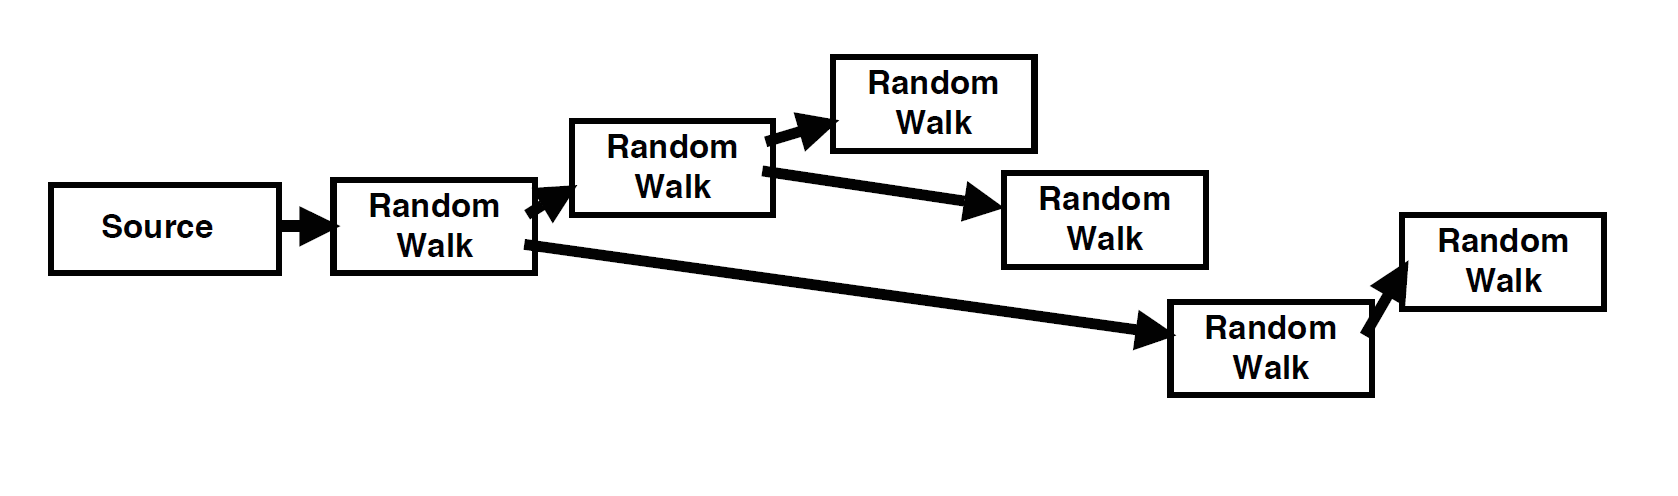
\includegraphics[width=0.75\textwidth]{walk - edited.png}
% \end{figure}
% In the diagram, some particle (a proton or a neutron, for example) starts its path at the source block and is launched in a random direction. After that, it can interact with something else in the simulation space - other protons or neutrons. A collision takes place and the particle is launched into another random direction. This goes on for a certain number of cycles, specified by the user.

%takes Monte-Carlo simulations one step forward. The program solves a series of random-walk problems. In the current case, a random particle is traced from its source to a certain definition.